\section{流体非压强力模型}
    第三章中通过位置约束的求解即可得到一个高效稳定的不可压缩流体的仿真框架。不过由于离散采样、近似误差等原因使得模拟效果真实感不强,产生了诸如粒子内聚力太低、粒子抖动、涡量不守恒等问题。本章将通过严谨的物理建模或启发式的经验公式来解决这些问题,比如表面张力、人工粘性、涡量补偿等。这些方法均在压强求解后计算,统称为非压强受力。这部分我们不再采用位置约束求解而是基于传统的物理定律,计算每种力产生的加速度,再通过时间积分改变粒子的速度与位置。
    
    \begin{figure}[htbp]
    	\centering
    	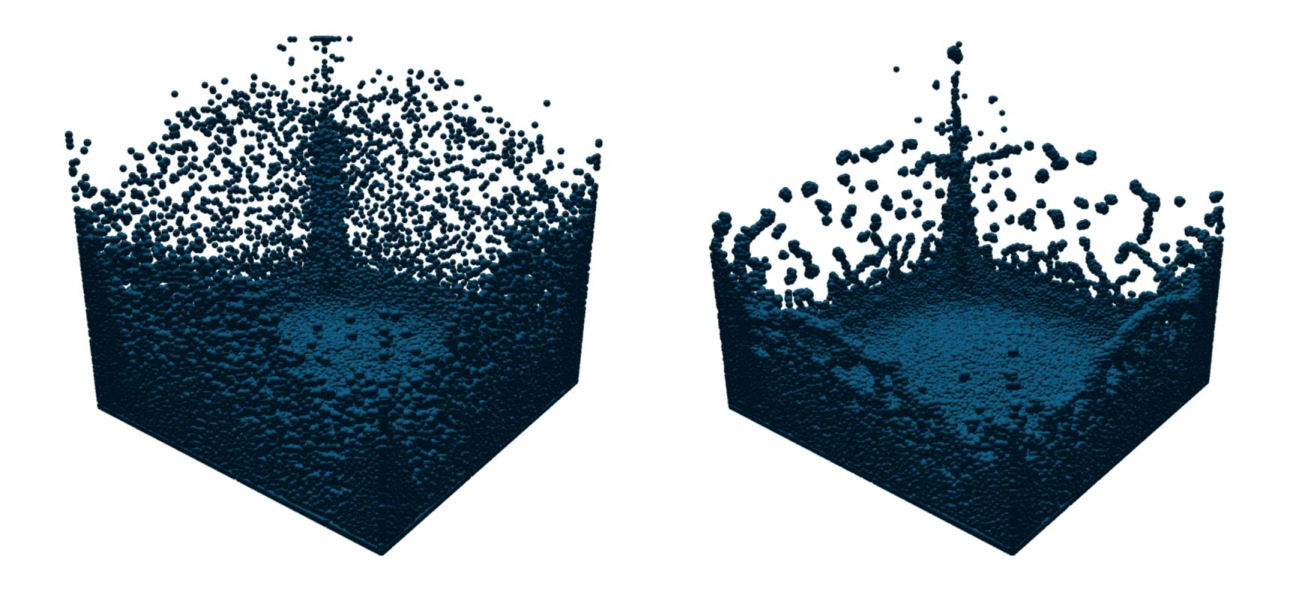
\includegraphics[width=.99\textwidth]{figures/simulation/tension.pdf}
    	\caption{关闭表面张力(左)开启表面张力(右)}
    \end{figure}

\subsection{表面张力}
    表面张力是一种重要的物理现象,在日常生活中普遍存在。它是微观尺度上液体分子间相互吸引的结果。分子在流体内部相互吸引,而表面的分子被向内拉。因此,表面张力会使流体表面积最小化,比如,当排除外力时水滴会形成球体(如图\ref{fig:tensionsphere})。Akinci等人\cite{AAT13SPH}在微观尺度计算粒子内聚力,宏观尺度最小化流体表面积,同时考虑这两种因素来建模流体表面张力。

\subsubsection{内聚力}
    粒子内聚力可以由粒子与其近邻粒子之间的位置差来确定,其计算公式为
    \begin{equation}
    	\mathbf F_{i \leftarrow j} ^{cohesion}
    	= - m_i m_j
    	\frac {\mathbf x_i - \mathbf x_j} {\mathbf x_i - \mathbf x_j}
    	W_{cohesion} (|\mathbf x_i - \mathbf x_j|)
    \end{equation}
    其中 $W_{cohesion}$ 是为计算内聚力而设计的特殊核函数,在采样点据核函数中心过近时会取得负值,在 $|\mathbf r| = 0.5h$ 时取得最大值。这样在粒子间距过小时产生排斥力,防止粒子聚集,而在其间距过大时内聚力趋近于0,对距离较远的粒子也没有影响,仅当粒子间距在一定范围内时,内聚力才有较大影响。其具体定义如下
    \begin{equation}
    	W_{cohesion}(\mathbf r, h) = \frac {32} {\pi h^9}
    	\left\{
    	\begin{array}{ll}
    
    	(h - |\mathbf r|)^3 |\mathbf r|^3 & 0.5h < |\mathbf r| \le h \\
    	2(h - |\mathbf r|)^3 |\mathbf r|^3 - \frac {h^6} {64} & 0 < |\mathbf r| \le 0.5h \\
    	0 & \mathrm{otherwise} \\
    
    	\end{array}
    	\right.
    \end{equation}
    
    \begin{figure}
    	\centering
    	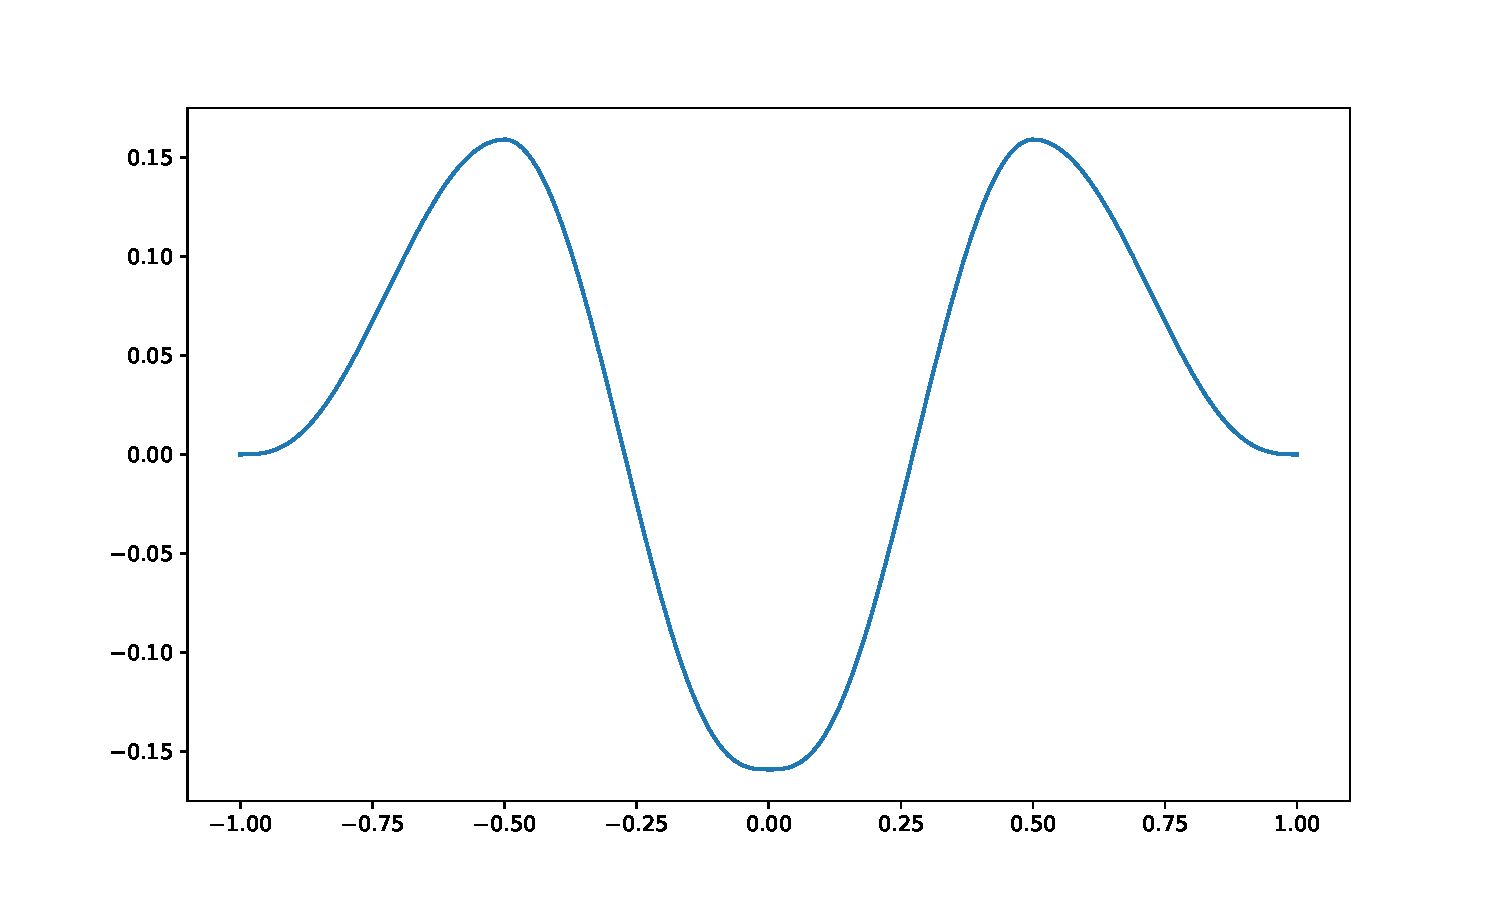
\includegraphics[width=.85\textwidth]{figures/simulation/cohesion_kernel.pdf}
    	\caption{内聚力核函数示意图}
    \end{figure}
    
    \begin{figure}[bp]
    	\centering
    	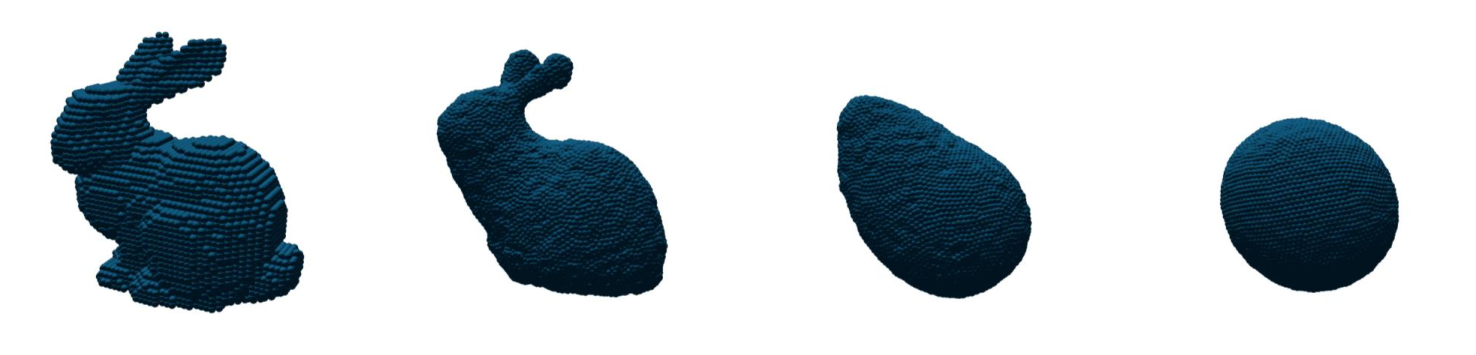
\includegraphics[width=.99\textwidth]{figures/simulation/surface.pdf}
    	\caption{流体粒子在没有重力的环境中形成球形}
    	\label{fig:tensionsphere}
    \end{figure}

\subsubsection{最小化表面积}
    在微观尺度上计算粒子内聚力仍不足以最小化流体表面积,因此Akinci等人设计了额外的力来抵消表面的曲率变化,定义如下
    \begin{equation}\label{eq:curvature}
    	\mathbf F_{i \leftarrow j} ^{curvature} =
    	- m_i (\mathbf n_i - \mathbf n_j)
    \end{equation}
    其中 $\mathbf n$ 为粒子法向。对于法向的计算,可以采样平滑颜色场的思路,具体来说,将粒子颜色设为1,而其他区域均记为0,那么计算这个平滑颜色场的梯度就可以得到此粒子的法向
    \begin{equation}
    	\mathbf n_i = h \sum_j \frac {m_j} {\rho_j} \nabla W_{ij}
    \end{equation}
    如果粒子在流体内部,显然上式计算结果趋近于0,而粒子在流体表面时,计算结果为指向表面外的向量,方向与表面曲率大小成正比。将其代入公式\ref{eq:curvature}可以发现,粒子受力在流体内部与较平整的流体表面计算结果均为0,曲率越大时,受力也越大。
    
    最终结合微观与宏观尺度的受力模型,表面张力计算公式为
    \begin{equation}
    	\mathbf F_{i} ^{surface\;tension} =
    	\alpha \sum_j K_{ij} (\mathbf F_{i \leftarrow j} ^{cohesion} + \mathbf F_{i \leftarrow j} ^{curvature})
    \end{equation}
    其中 $\alpha$ 为用户指定的表面张力参数,$K_{ij} = \frac {2\rho_0} {\rho_i + \rho_j}$ 是一个对称的缩放因子,在密度计算值偏低的流体表面放大表面张力的影响。

\subsection{涡量补偿}
    湍流是流体运动中最具视觉吸引力的现象之一,它是由于不同尺度上流体速度场的涡量产生的。在密度约束解算中,会引入许多额外的阻尼,产生能量耗散,所以流体速度场涡量也往往难以保持。Macklin等人\cite{MM13PBF}采用涡量补偿(Vorticity Confinement)的方法对流体系统注入额外能量
    \begin{equation}
    	\mathbf F_i ^{vorticity} =
    	\gamma (\frac{\eta_i}{|\eta_i|} \times \omega_i) \\
    	\eta_i = \nabla |\omega_i| = \sum_j \frac {m_j} {\rho_j} |\omega_j| \nabla W_{ij}
    \end{equation}
    其中 $\omega$ 为涡量,其计算公式如下
    \begin{equation}
    	\omega_i = \nabla \times \mathbf v =
    	\sum_j \mathbf v_{ij} \times \nabla W_{ij}
    \end{equation}
    
    \begin{figure}[htbp]
    	\centering
    	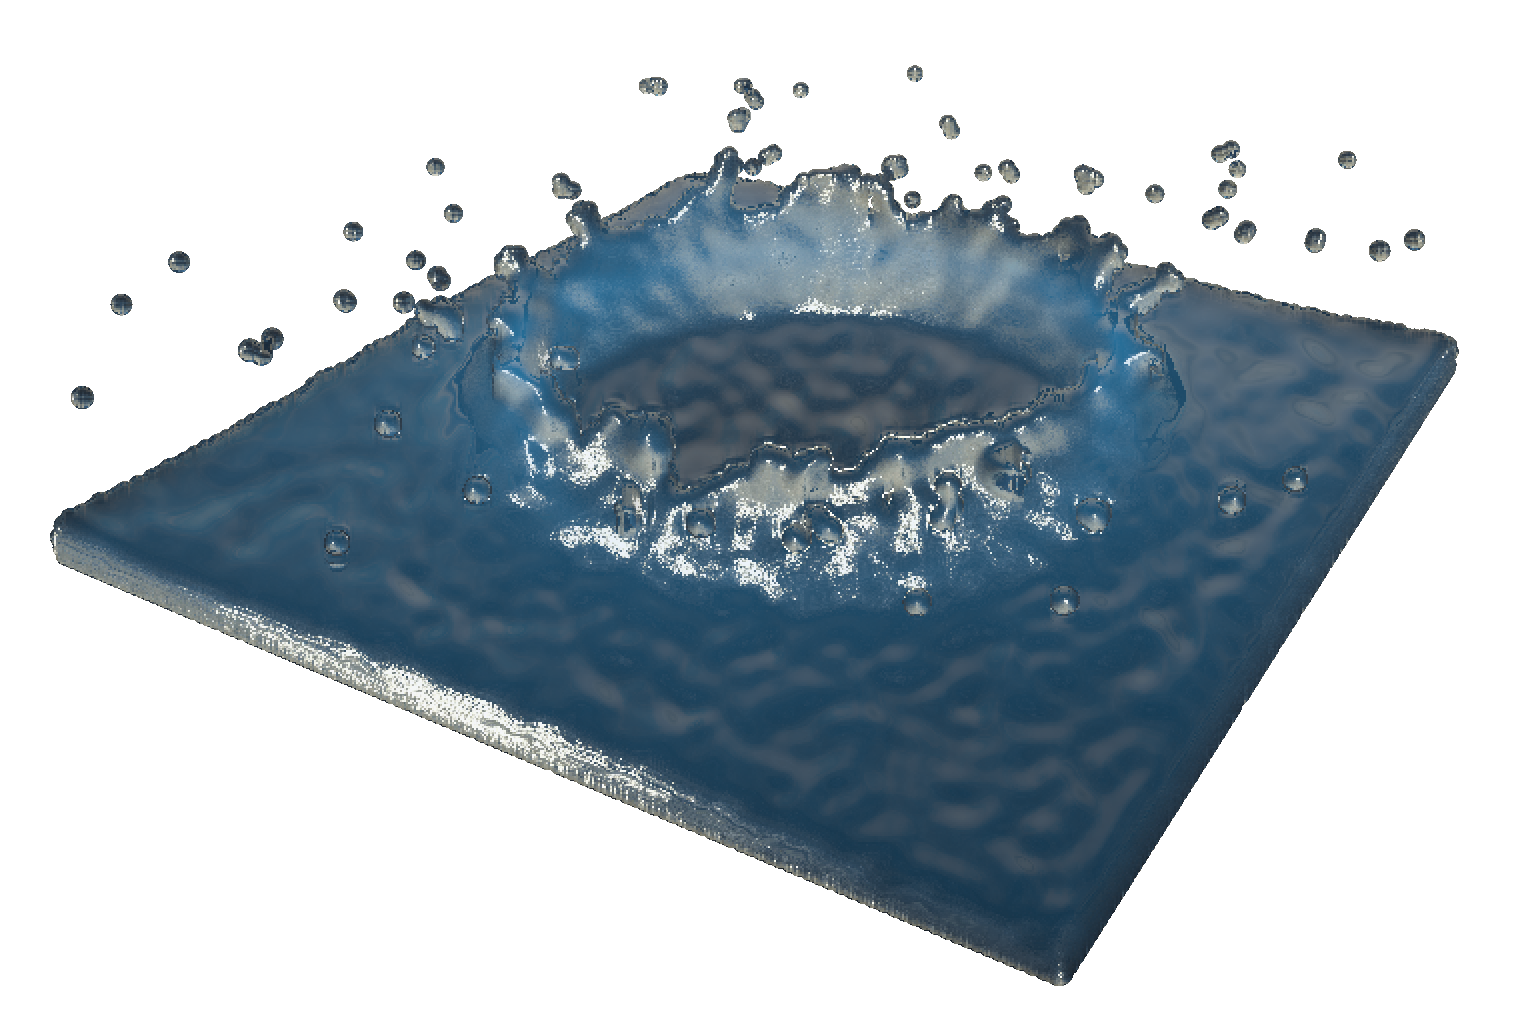
\includegraphics[width=.7\textwidth]{figures/simulation/drop.png}
    	\caption{在非压强力作用下的水滴掉落场景}
    \end{figure}

\subsection{人工粘性}
    PBF的位置约束推导是以密度不变为核心的,理论上这相当于速度场散度为0,即满足流体不可压缩条件。但在实际计算过程中,由于没有对流体速度场做相应约束,会导致速度场中存在高频噪声,反应到模拟效果上就是流体粒子在不停地小幅震动。Bender等人提出的DFSPH\cite{BK15DFSPH}方法通过同时求解密度和速度散度这两个约束条件完全解决了这个问题。但出于性能考虑,本文通过引入人工粘性XSPH\cite{SB2012XSPH}来缓解这种现象,简单来说,XSPH相当于对流体速度场做了一次模糊操作,减少了高频噪声,其计算过程如下
    \begin{equation}
    	\mathbf v_i' = \mathbf v_i + \beta \sum_j \mathbf v_{ij} \cdot W_{ij}
    \end{equation}
    其中 $\beta$ 为指定的粘性系数,$\mathbf v_{ij}$ 为粒子间速度之差,即 $\mathbf v_{ij} = (\mathbf v_i - \mathbf v_j)$ 。这种显示更新速度的方式在时间步较大时并不稳定,所以人工粘性只适用于水这种几乎没有粘性的流体,而蜂蜜等高粘性流体需要隐式积分的处理方式。

\subsection{本章小结}
    本章主要阐述了SPH框架中三种非压强力,分别是表面张力、涡量补偿力与粘性力。其中本章从宏观和微观两种角度下分别推导了对应的约束力公式,组合在一起形成表面张力公式。而涡量补偿本质上是向系统中注入新的能量用于抵消数值计算产生的阻尼,保证了流体速度场涡量守恒。最后,粘性力用于去除流体速度场的高频噪声,防止粒子抖动。这些非压强受力均在流体压强解算后施加,用于增强流体仿真的真实感和稳定性。